\documentclass[a4paper]{article}
\usepackage{amsfonts}
\usepackage{amsmath}
\usepackage{amssymb}
\usepackage{graphicx}      

\newcommand{\dint}{\displaystyle\int}

\begin{document}
  
\noindent \large Auteur: Thijs Van Schel \\
\noindent \large Studierichting: Informatica\\
\noindent \large Oefeningenreeks 5G nr. 17\\

\medskip

\normalsize

$y^2 = 4x \Rightarrow x = \dfrac{y^2}{4}$\\

snijpunten met $x = 1$:\\

$y^2 = 4 \cdot 1 \Rightarrow y^2 = 4 \Rightarrow y = -2$ of $y = 2$\\

omwenteling rond $x = 1$, integratie naar $y$:\\

$V = \pi \dint_{-2}^{2} (1 - x)^2 dy$\\

$= \pi \dint_{-2}^{2} \left(1 - \dfrac{y^2}{4}\right)^2 dy$\\

$= \pi \dint_{-2}^{2} \left(1 - \dfrac{y^2}{2} + \dfrac{y^4}{16}\right) dy$\\

$= \pi \left[ y - \dfrac{y^3}{6} + \dfrac{y^5}{80} \right]_{-2}^{2}$\\

$= \pi \left( \left(2 - \dfrac{8}{6} + \dfrac{32}{80}\right) - \left(-2 - \dfrac{-8}{6} + \dfrac{-32}{80}\right) \right)$\\

$= \pi \left( \left(2 - \dfrac{4}{3} + \dfrac{2}{5}\right) - \left(-2 + \dfrac{4}{3} - \dfrac{2}{5}\right) \right)$\\

$= \pi \left( 4 - \dfrac{8}{3} + \dfrac{4}{5} \right)$\\

$= \pi \left( \dfrac{60}{15} - \dfrac{40}{15} + \dfrac{12}{15} \right)$\\

$V = \dfrac{32\pi}{15}$\\

tekening:\\

\begin{figure}[h]
    \centering
    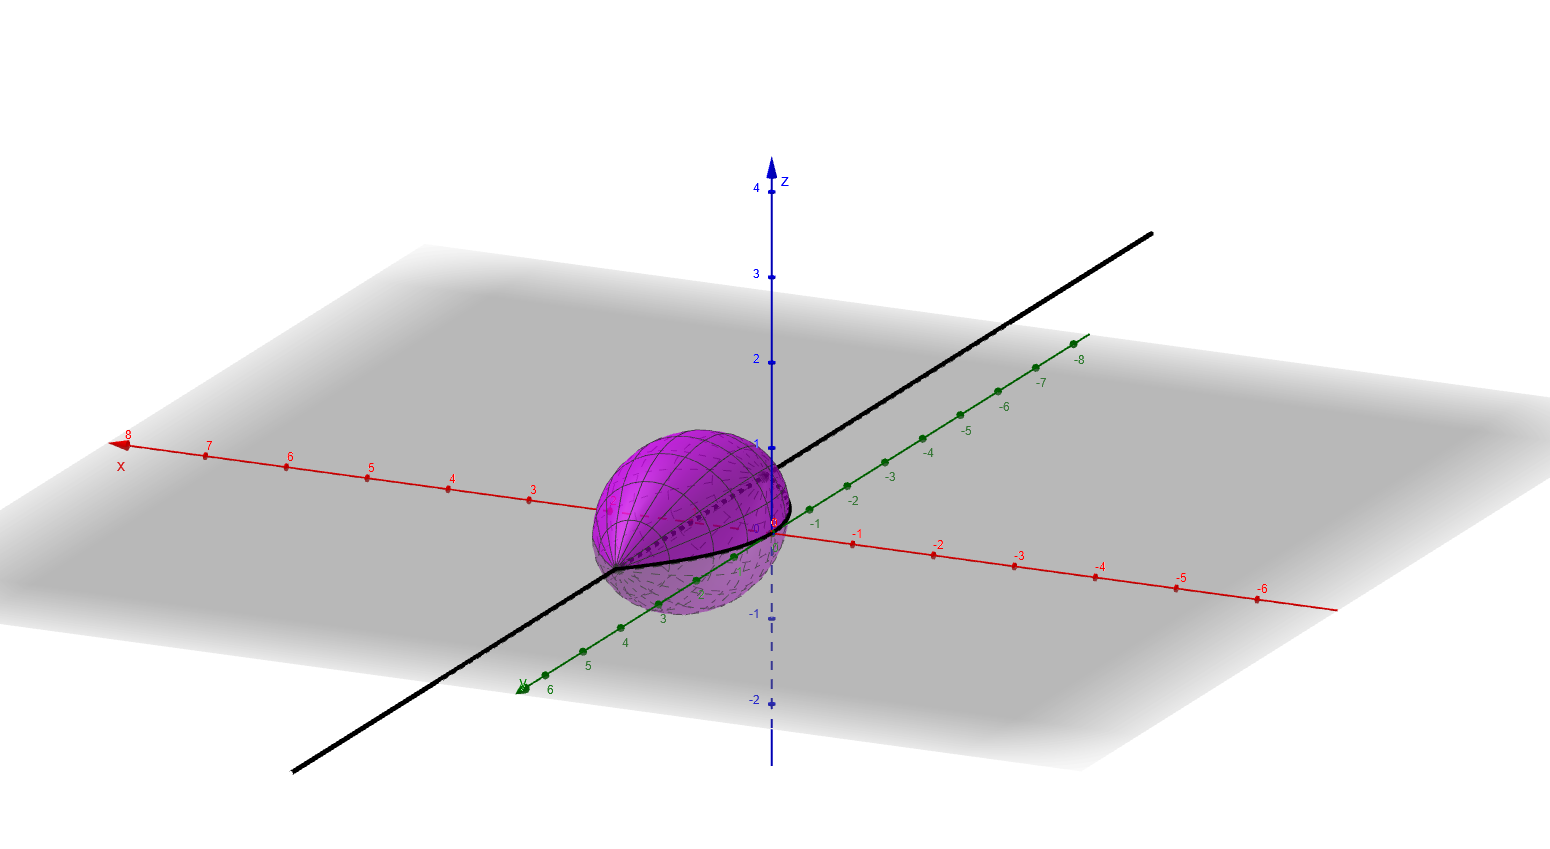
\includegraphics[width=0.6\textwidth]{5G-17-thijs.van.schel.INF.png}
\end{figure}

\begin{thebibliography}{999}
%\bibitem{a} Referentie
\end{thebibliography}
\end{document}